%\documentclass[]{AIAA}
%\begin{comment}
\documentclass[%
 aip,
%jmp,%
%bmf,%
%sd,%
rsi,%
 amsmath,amssymb,
%preprint,%
 reprint,%
%author-year,%
%author-numerical,%
]{revtex4-1}
%\end{comment}
\usepackage{amsmath}
\usepackage{amssymb}
\usepackage{graphicx}
\usepackage{verbatim}
\usepackage{placeins}
\usepackage{multirow}
\usepackage{epstopdf}
%\usepackage[font=bf,justification=justified,format=plain]{caption}
%\usepackage{hyperref}
%\usepackage{authblk}
%\usepackage{setspace}
\usepackage{natbib}
\bibliographystyle{unsrtnat}




\begin{document}
\title{Improvements to the Ion Doppler Spectrometer Diagnostic on the HIT-SI Experiments}

%\author{ \large{Rian Chandra\footnote{rianc@uw.edu}, Aaron Hossack, Tom Jarboe}\\ \small{University of Washington, Seattle, WA, USA}}
\author{Rian Chandra}\email{rianc@uw.edu}\affiliation{University of Washington, Seattle, WA, USA}
\author{Aaron Hossack}\affiliation{University of Washington, Seattle, WA, USA}
\author{Tom Jarboe}\affiliation{University of Washington, Seattle, WA, USA}
\author{Chris Everson}\affiliation{University of Washington, Seattle, WA, USA}
\begin{abstract}
An Ion Doppler Spectrometer diagnostic system has been constructed to measure impurity ion temperature and velocity on the HIT-SI and HIT-SI3 spheromak devices with improved spatiotemporal resolution and lower error. Hardware and software improvements have resulted in a record $6.9\,\mu$s temporal and $\leq2.8$ cm spatial resolution in the midplane of the devices. With these, C III and O II flow, displacement, and temperature profiles can be simultaneously observed.  With 72 fused-silica fiber channels in two independent bundles, and an f/8.5 Czerny-Turner spectrometer coupled to a CCD, frame-rates of up to ten times the applied perturbation frequency of 14.5 kHz were achieved in HIT-SI, viewing the upper 1/2 of the midplane. In HIT-SI3 frame-rates of up to eight times the perturbation frequency were achieved viewing both halves of the midplane. Biorthogonal Decomposition is used as a novel filtering tool, reducing uncertainty in ion temperature from $\lesssim13$ to $\lesssim5$ eV with an instrument temperature of 8-16 eV, and uncertainty in velocity from $\lesssim2$ to $\lesssim1$ km/s. Errors are calculated using the Levenberg-Marquart algorithm. Axisymmetric temperature profiles on HIT-SI3 for C III peaked near the inboard current separatrix at $\approx40$ eV are observed. Axisymmetric plasma displacement profiles have been measured on HIT-SI3, peaking at $\approx6$ cm at the outboard separatrix. Both profiles agree with the upper half of the midplane observable by HIT-SI. With its complete midplane view, HIT-SI3 has unambiguously extracted axisymmetric, toroidal current dependent rotation of up to 3 km/s. Analysis of the temporal phase of the displacement uncovers a coherent structure, locked to the applied perturbations. 
%Analysis is presented for O-II and C-III, for both toroidal current directions. 
\end{abstract}
\keywords{Ion Doppler Spectrometer, HIT-SI, Plasma Diagnostics, Spheromak}
\renewcommand{\thefootnote}{\roman{footnote}}
\maketitle
%\singlespacing
%%%%%%%%%%%%%%%%%%%%%%%%%%%%%%%%%%%%%%%%%%%%%%%%%%%%%%%%%%


%%%%%%%%%%%%%%%%%%%%%%%%%%%%%%%%%%%%%%%%%%%%%%%%%%%%%%%%%%%
\section{Motivation}
\hspace{4ex}Accurate measurements of ion velocity and temperature play an important role in understanding fusion plasma experiments. In the HIT-SI and HIT-SI3 spheromak devices, it is anticipated that the MHD dynamo term will play a large role in the magnetic self-organization process. Furthermore, toroidal ion rotation and radial velocity shear both play important roles in stabilization and the suppression of instabilities in the plasma. Ion temperature is necessary to calculate $\beta_{plasma}$ ($\beta_p = \frac{P_{thermal}}{B^2/2\mu_o}$), and for the calculation of various characteristic timescales. It is anticipated from numerical simulation\cite{akcay2013extended} that the chord-averaged ion velocities will be of order $10$ km/s, and from both simulation and Langmuir probe measurements that the ion temperatures will be of order $10$~eV. Because the signal to noise ratio in this regime is likely to be small, characterization of error is required, as is signal filtering. The demands on spatio-temporal resolution are set by the period of the imposed perturbation (69 $\mu$s), and relatively small major radius (55 cm). Temporally, data must be collected for the majority of the shot, at sub-perturbation resolution. Spatially, we wish to observe as much of the toroidal midplane as possible, with multiple spatial chords. Previously reported diagnostic systems cannot fulfill these demands simultaneously: Cochran \cite{cothran2006fast} describes an Ion Doppler Spectrometer (IDS) diagnostic on SSX with 1 $\mathrm{\mu}$s temporal resolution and low error ($\leq6$ km/s, $\leq7$ eV), but only one spatial channel. Baciero \cite{Baciero2001JT-II} describes an IDS system on TJ-II with 8 chords at $\leq5$ cm spatial resolution across the entire poloidal plane, but only 15 ms temporal resolution. Bamford \cite{bamford1992combination} on the COMPASS-C tokamak and den Hartog \cite{den1994fast} on the MST RFP are further examples of systems with insufficient spatio-temporal resolution. The IDS diagnostic reported here addresses these requirements. An overview of the experimental and diagnostic hardware will be presented, followed by the analysis and filtering techniques used to calculate the final results.



%%%%%%%%%%%%%%%%%%%%%%%%%%%%%%%%%%%%%%%%%%%%%%%%%%%%%%%%%%%
\section{The HIT-SI and HIT-SI3 Devices}
\hspace{4ex}The HIT-SI\cite{sieck2005initial} and HIT-SI3\cite{Hossack_HitSi3} experiments study spheromak sustainment via the injection of magnetic helicity into a simply-connected flux conserver. The helicity injectors (on Fig.\ref{Fig::V-Tank}) are driven at a fixed frequency (14.5 kHz for this work), and phased such that the rate of helicity injection is constant. In the data presented here, phasing is set to  $\Delta\phi=120^\circ$ for HIT-SI3 and $\Delta\phi=90^\circ$ for HIT-SI. The theoretical basis for steady state sustainment is given by the theory of ``Imposed Dynamo Current Drive''\cite{jarboe2012imposed}. The experiments' diagnostic set includes: a far infrared laser interferometer (reporting $1\times10^{19}\lesssim{n_e}\lesssim8\times10^{19}$  m$^{-3}$)\cite{hossack2013reduction}, a Langmuir probe (reporting electron temperatures $T_e\lesssim10$ eV)\cite{ONeil2007experimental}, and an array of toroidal and poloidal magnetic field probes in the wall which allow mode reconstruction up to toroidal Fourier number $n=7$\cite{Oneil2007overview}. Gas fueling is controlled by solenoid valves. Toroidal current, injected power, helicity injection rate, and electron density are shown in Fig \ref{Fig::Jscope}. The flux conservers for both experiments are pictured in figure \ref{Fig::V-Tank}.
\begin{figure*}
\includegraphics[width=6in]{V_Tank}\caption{HIT-SI3 (left) and HIT-SI (right) flux conservers cut away at the toroidal midplane. Helicity injectors are shown, with flux coils (blue on HIT-SI and white on HIT-SI3) and voltage coils (red on HIT-SI and multicolored on HIT-SI3) shown separately. On HIT-SI, the second injector (`Y') opposes the pictured one (`X'), rotated 90$^\circ$ toroidally. On HIT-SI3, all injectors (`A',`B', and `C') are pictured. }\label{Fig::V-Tank}
\end{figure*}

%\FloatBarrier

%%%%%%%%%%%%%%%%%%%%%%%%%%%%%%%%%%%%%%%%%%%%%%%%%%%%%%%%%%%
\section{Diagnostic Process}
\hspace{4ex}The use of IDS diagnostics for fusion plasma experiments is common\cite{den1994fast}. The Doppler shift and broadening of impurity ion spectral lines from the plasma are correlated to the velocity and thermal motion respectively, along the viewing chord. Formally, \\
\begin{equation}\label{Doppler_Eqns}
v_i = c\frac{\Delta\lambda}{\lambda}\,\,\,\mathrm{[m/s]},\qquad
T_i = \frac{\sigma^2c^2m_i}{\lambda_0^2k_b}\,\,\,\mathrm{[eV]}
\end{equation} 
Where $\Delta\lambda$ is the shift in wavelength away from a calibration value, and $\sigma$ is the line width. The passive IDS system described here is in contrast to active systems, such as \cite{mckee1999beam}, \cite{fonck1984determination}, or \cite{burgos2012hybrid}. The HIT-SI and HIT-SI3 experiments assume that $||\vec{E}||$ and $||\vec{B}||$ are sufficiently low that the Stark, Zeeman, and other higher order effects will not measurably affect the spectral profile. This study primarily looks at line radiation from the $1s^22s3P\Rightarrow1s^22s3s$ 464.74 nm C III transition, and the $2s^22p^2(3P)3p\Rightarrow2s^22p^2(3P)3s$ 464.91 nm O II transition. C III impurity ions in particular are commonly observed due to their relative abundance across all impact parameters in medium-temperature plasmas\cite{cothran2006fast}. Both of these lines are the brighter components of doublets. 

%%%%%%%%%%%%%%%%%%%%%%%%%%%%%%%%%%%%%%%%%%%%%%%%%%%%%%%%%%
\section{Experimental Setup}
\subsection{Optical Hardware}
\hspace{4ex}The IDS hardware has been used on two iterations of the HIT-SI experiment. The following is quoted at length from  Hossack \cite{hossack2015study}. The spectrometer itself is a one-meter focal length Ritsu Ohyo Kogaku model MC-100N Czerny-Turner configuration grating monocrometer. The wavelength range is 250-700 nm and the focal ratio is f/8.5. The manually adjustable grating is blazed at 250 nm, and has a groove density of 1800 per mm. The adjustable entrance slit width is usually kept at 80~$\mu$m.\\
\hspace*{4ex}Light is gathered by two linear bundles of 36 channels, each 3 m long and insertable into several reentrant ports on the vacuum vessel. Plasma light is imaged onto the fibers by a wide angle ``Micro Video Lens'' from Edmund Optics, with a focal length of 2.2 mm. Each fiber channel therefore collects a conical volume of plasma light, of radius 5.1 cm at 110 cm, the vacuum vessel diameter. The chords are separated by 2.95$^{\circ}$.\\
\hspace*{4ex}The spatial extent of the IDS light collection optics is significantly larger and more mutable than that of previously described experiments (such as \cite{cothran2006fast},\cite{Baciero2001JT-II}, or \cite{den1994fast}). Figure \ref{Fibers Midplane} shows the configurations used in this report. There exists radial and opposing poloidal viewports as well. The ability to view the upper and lower halves of the toroidal midplane simultaneously is an improvement not seen on other devices.
\begin{center}
\begin{figure}
%\includegraphics[width=3in]{HITSI_Midplane.jpg}
%\caption{HIT-SI Midplane fiber array: radial port (left), upper 1/2 midplane port (right)}\label{HIT-SI Fibers Midplane}
\includegraphics[width=3.0in]{Mohawk_IDS_dual.png}
\caption{Midplane fiber arrays: only the upper (green) array was installed on HIT-SI. HIT-SI3 could view above and below the geometric axis. Chords are superposed over the HIT-SI3 injectors, with `A' vertical on the right, `B' on the upper left, and `C' on the lower left. The red ring is the approximate magnetic axis.}\label{Fibers Midplane}
%\includegraphics[width=3in]{Untitled.jpg}
%\caption{HIT-SI Poloidal fiber array (left), velocity-zeroing configuration (right)}\label{Fibers Poloidal}
\end{figure}
\end{center}
\subsection{Camera and Calibration}
\hspace*{4ex}The output of the spectrometer is optically coupled to a Phantom v710 Fast Camera. Previous studies found the trade-off between temporal resolution and detection channels in PMTs vs. CCDs respectively not favorable (Bamford on the COMPASS-C tokamak \cite{bamford1992combination} utilizes both to circumvent this, for example), but this does not hold in the HIT-SI parameter regime. The camera has been run up to 145,000 pictures per second (10 frames per injector cycle, 6.9 $\mu$s exposure) for high-current discharges, with acceptably low error (see sec. \ref{sec:Fit}). \\
\hspace*{4ex} A mercury lamp, viewed through a ground glass diffuser, is used to evenly illuminate the fibers. Spectral lines close to the plasma impurity lines of interest are chosen (in this case, the doublet 434.75 and 435.84 nm) to account for nonlinearity in the grating. An elliptical Gaussian of the form in Eqn.~\ref{Eqn::Gaussian} is fit to the brightest line:
\begin{eqnarray}\label{Eqn::Gaussian}
f(x,y,a)=\frac{V}{2{\pi}\sigma_x\sigma_y}\times\nonumber\\ exp\left(-\frac{1}{2}\left(\frac{(x-x_0)^2}{\sigma_x^2}+\frac{(y-y_0)}{\sigma_y^2}\right)\right)+f_0
\end{eqnarray}
where $x$ and $y$ are the spatial and wavelength directions, respectively, and `$a$' encapsulates the parameters: ${\sigma}_x$ is the spatial width, ${\sigma}_y$ is the wavelength width, $x_0$ and $y_0$ are the spatial and wavelength centers respectively, and $f_0$ is the background (continuum) offset level. This is done to calibrate the instrument function ($\sigma_y$), which corresponds to an instrument temperature between 8-16 eV for C III), position ($x_0,y_0$), and relative intensity ($V$). By tuning the spectrometer with a stepper motor, the doublet can be used to calculate the dispersion (wavelength-per-pixel). To avoid nonlinearity in the exit optics, only dispersion values near the center of the CCD are used.  Because the calibration line is not near the plasma lines (465 nm), the absolute velocity cannot be established with this calibration. An example of the raw data collected by the camera is given in Fig \ref{HITSI_CCD}.
\begin{center}
\begin{figure*}
\centering
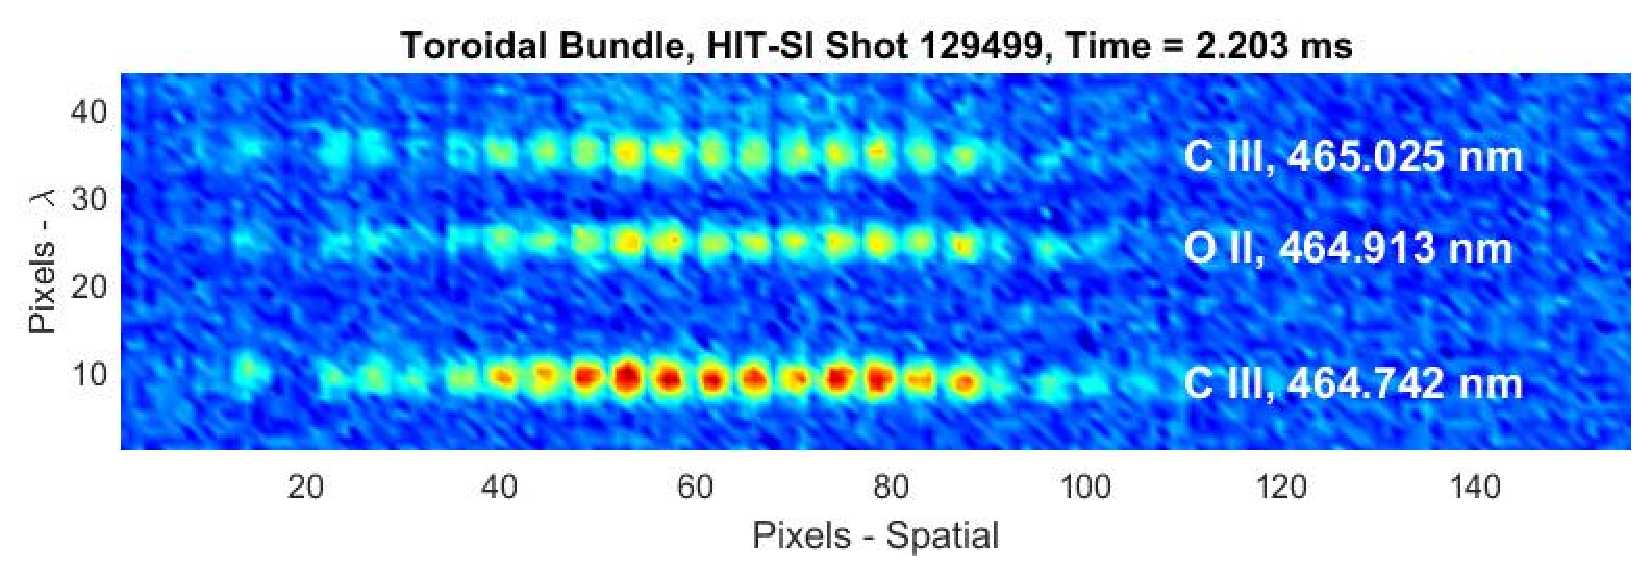
\includegraphics[width=6in]{HITSI_CCD_3}\caption{Raw CCD image from HIT-SI shot 129499, C III \& O II. Pictured data from upper 1/2 midplane port (Fig. \ref{Fibers Midplane}). Second array in poloidal port not pictured. Intensity units arbitrary. }\label{HITSI_CCD}
\end{figure*}
\end{center}

%%%%%%%%%%%%%%%%%%%%%%%%%%%%%%%%%%%%%%%%%%%%%%%%%%%%%%%%%

\section{Biorthogonal Decomposition Filtering of Raw Data}\label{sec::BD}
\hspace{4ex}The low SNR in figure \ref{HITSI_CCD} motivates the use of a filtering algorithm. Because the temporal evolution of the data is not known \textit{a priori}, it is preferable to use a method which does not impose pre-determined basis functions (such as the Fourier transform). Singular Value Decomposition (SVD) meets this requirement. The technique has been applied frequently to the decomposition of MHD mode activity from magnetic field measurements (first by de Wit \cite{de1994biorthogonal}, first on HIT-SI by Brian Victor\cite{BVictor}), but has been used on IDS systems as well \cite{fenzi20012d}. The technique, frequently referred to as Biorthogonal Decomposition (BD), is unique in that the basis functions are determined by the data itself. Each frame on the CCD is collapsed into a single vector, and these vectors are concatenated to convert the 3D data of dimensions wavelength $\times$ space $\times$ time into a 2D matrix of dimension pixel $\times$ time, which can then be analyzed. It can be shown\cite{kutz2013data} that any matrix B is guaranteed a singular value decomposition, resulting in Eqn \ref{Eqn::BD}.
\begin{equation}\label{Eqn::BD}
B(x_m,t_n)= \sum^K_{k=1}\phi_k(x_m)A_k\psi_k^T(t_n) = U\Sigma{V^*}
\end{equation}
The traditional SVD notation is given on the right, and the BD notation in the middle. The data can be fully reconstructed by summing over all $K$ ``modes'', where $\phi$ and $U$ are the $m\times{m}$ orthonormal spatial basis structures (``topos''), $A$ and $\Sigma$ are the diagonal matrix of singular values (``weights''), and $\psi^T$ and $V^*$ are the orthonormal temporal basis structures (``cronos''). While other experiments have studied these structures (such as the ``cronos'' given in Fig.\ref{BD Weight}b) themselves\cite{fenzi20012d}, this paper uses BD as solely a filtering tool, in which the data is reconstructed from a minimum number of modes. Figure \ref{BD Weight}a shows the magnitudes of the weights. We truncate the dataset at mode ten, with the rest of the modes being considered noise (other studies have proposed data reconstruction with even fewer modes\cite{gavish2014optimal}). We can capture up to approximately $80\%$ of the modal energy (calculated as $A_k^2$ \cite{de1994biorthogonal}) in this way. This has a significant effect on the uncertainty in velocity and temperature (calculated in sec. \ref{sec:Fit}), shown in figure \ref{BD Uncertainty}. A comparison of the raw data and reconstruction is shown in figure \ref{BD CCD}. To qualitatively confirm that valuable data is not discarded, a reconstruction is made from the discarded modes, a frame from which is plotted in figure \ref{BD Noise}. No residual structure is observed.
\begin{center}
\begin{figure*}
\includegraphics[width=6in]{BDWeight_1}\caption{BD weights 1-30 (a). Dominant ``cronos'' showing background and oscillatig modes (b). HIT-SI shot: 129499 \cite{hossack2015study}}\label{BD Weight}
\end{figure*}
\begin{comment}
\begin{figure}
\includegraphics[width=6in]{BDTopos}\caption{BD dominant ``topos'', HIT-SI shot: 129499}\label{BD Topos}
\end{figure}
\end{comment}
\begin{figure*}
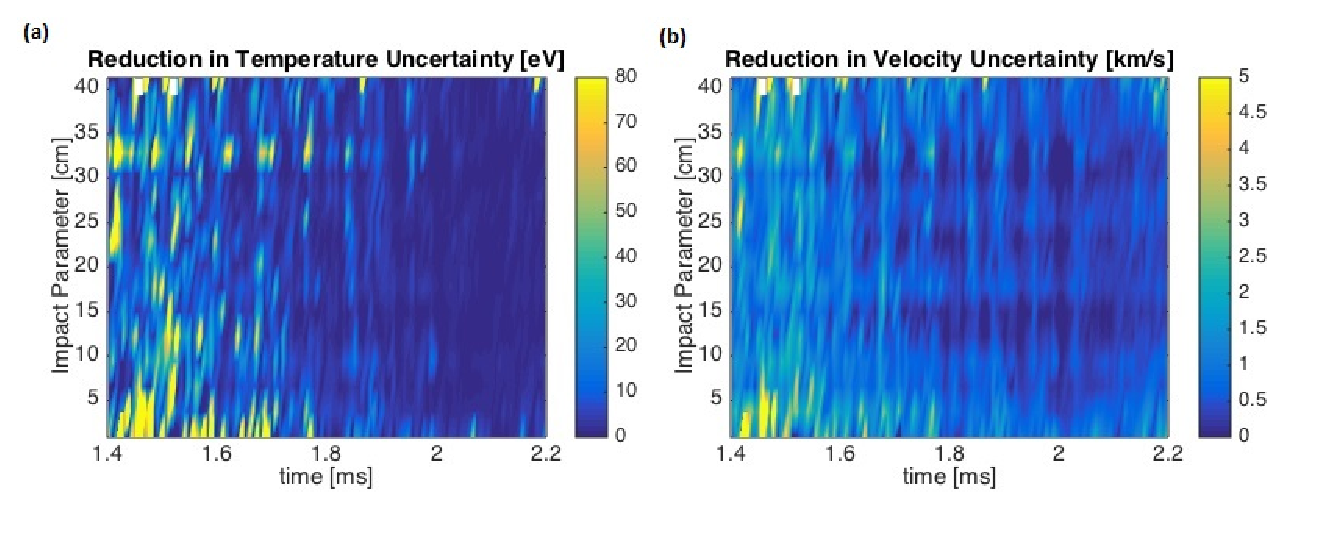
\includegraphics[width=6in]{BD_Uncertainty_1}\caption{(A): Post BD filtering reduction in temperature and (B): velocity uncertainty. HIT-SI shot: 129499 \cite{hossack2015study}.}\label{BD Uncertainty}
\end{figure*}
\begin{figure*}
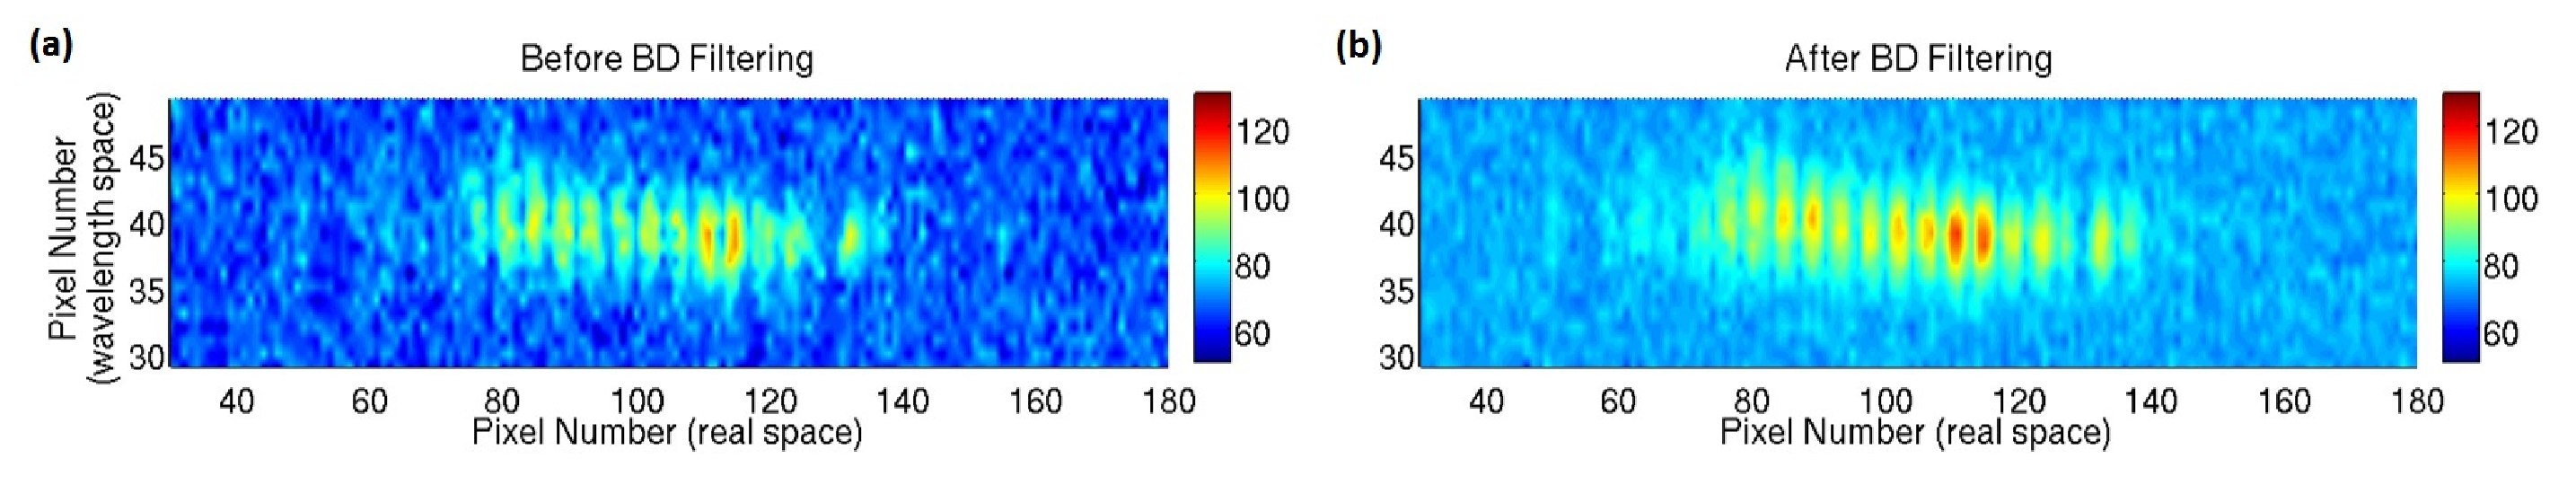
\includegraphics[width=6in]{CCD_BD_1}\caption{Raw CCD before (a) and after (b) BD filtering, HIT-SI shot: 129499, time 1.437 ms \cite{hossack2015study}. Intensity arb.}\label{BD CCD}

\end{figure*}
\begin{figure}
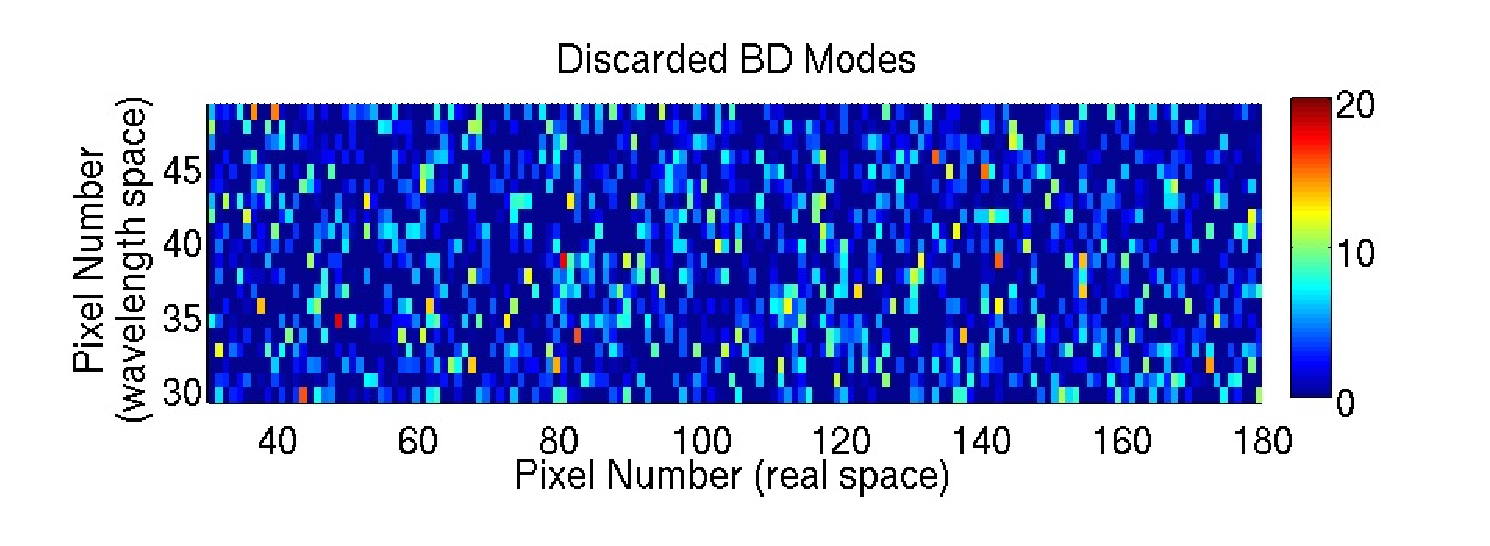
\includegraphics[width=3.5in]{BD_Discard}\caption{Noise reconstruction CCD frame, HIT-SI shot 129499, time 1.437 ms \cite{hossack2015study}. Intensity arb.}\label{BD Noise}
\end{figure}
\end{center}


%%%%%%%%%%%%%%%%%%%%%%%%%%%%%%%%%%%%%%%%%%%%%%%%%%%%%%


\section{Fitting to the Data}\label{sec:Fit}
\subsection{Fit Function}
An elliptical gaussian function of the form of Eqn. \ref{Eqn::Gaussian} is fit to each channel at each timepoint. It should be noted that in similar spectroscopic studies, fitting to a 1D gaussian is typical. \begin{comment}{For research using a PMT as the photon counter (such as \cite{cothran2006fast}), 1D fitting is usually a necessity, however,\end{comment}
For studies using a CCD (\cite{den1994fast}\cite{rapisarda2007role}\cite{bamford1992combination}), where light falls onto a 2D grid of pixels, gaussians are either binned in the spatial direction or treated as if light falls only on a single column of pixels. In this system, light for each channel covers 2-3 pixels spatially (Fig \ref{HITSI_CCD}), so if the fiber alignment is shifted slightly (eg: the spectrometer is bumped), an $x_0$ fixed to the calibration value will result in an artificially reduced $\sigma_y$, and therefore reduced temperature and worse fit. We eliminate this source of error by allowing $x_0$ to vary as a free parameter to keep the fit centered on the data. $\Delta{x_0}$ corrections of up to $\pm26\%$ of $\sigma_x$ are observed.\\


\subsection{Levenberg-Marquart Fitting}\label{sec::LM}
\hspace*{4ex}The model function $f(x,y,a)$ (Eqn \ref{Eqn::Fit_Fn}) is fit to the data using the Levenberg-Marquardt Method (LMM). This has been used in other plasma diagnostics to fit nonlinear or convolved models to data, see citations \cite{Nikolić200167}\cite{Heesterman}\cite{Avdeeva}\cite{Pablant}\cite{Reinke}\cite{Luxon} or \cite{Lazerson}\\
\hspace*{4ex}The LMM, as derived independently by K. Levenberg\cite{LEVENBERG} and D. Marquardt\cite{marquardt1963algorithm}, combines the classical minimization techniques of linearizion (known alternately as the Taylor expansion method or the Gauss-Newton method):
\begin{eqnarray}\label{Eqn::G-N}
\delta{a} = -[J^TJ(x_k)]^{-1}\nabla{\chi^2} \nonumber\\ = -[J^TJ(x_k)]^{-1}{J^T}(F-f(x,y,a))
\end{eqnarray} 
and ``steepest descent'' (or, the gradient method):
\begin{equation}\label{Eqn::Grad}
\delta{a} = \alpha\times\frac{\partial\chi^2}{\partial{a}} = \alpha\times{J^T}(F-f(x,y,a)).
\end{equation}
The former is used when the model has converged close to the solution, the latter when it is farther away. The LMM has been shown to have quadratic convergence\cite{Fan2005} under the relatively weak condition that $||F-f(x,y,a)||$, where F is the data, provides a local error bound. Used alone, Taylor expansion is invalid when the initial guess is far from optimal, as quadratic linearizion of the model is no longer a valid reconstruction. Similarly, Gradient descent converges slowly when close to optimal, as the derivatives of the minimizing function $\chi$:
\begin{equation}\label{Eqn::Chi}
\chi^2 = \frac{1}{2}||F-f(x,y,a)||^2
\end{equation}
 are nearly zero (the Jacobian becomes rapidly singular). The unweighted LMM algorithm is implemented in Eqn \ref{Eqn::LM} \cite{press1996numerical}\cite{nocedal2006numerical}:\\
\begin{equation}\label{Eqn::LM}
(J^TJ+\lambda{I})\delta{a}=-J^T(F-f(x,y,a)).
\end{equation}
The iteration proceeds with an initial $\lambda=0.001$, and then increasing or decreasing by a factor of ten if the new value of $\chi^2$ is greater or smaller than the previous, respectively. The updated parameter is $\delta{a}$, $\alpha$ is a constant, and $J$ is the Jacobian matrix. 

\hspace*{4ex}A further attractive property of this implementation of the LMM is that it lends itself readily to the calculation of errors, not only of the overall model, but the standard parameter error as well. This ability to individually specify the errors in temperature and velocity represents a significant improvement over previous error propagation schemes in IDS instruments, which appear limited to RMS error, or S/N values. This is accomplished by approximating the covariance matrix of the final fit $f'$. Here, the Hessian matrix $\mathcal{H}$ is approximated by $[J^TJ]$ (where $J$ has already been calculated), assuming small higher order residuals\cite{yuen2010bayesian}:
\begin{eqnarray}
\sigma_P^2 =\mathrm{diag(covariance(f'))}= \mathrm{diag}(\sigma_{RMS}\mathcal{H}^{-1})\nonumber\\ = \mathrm{diag}(\sigma_{RMS}[J^TJ]^{-1}).
\end{eqnarray}
The sensitivity of the model with respect to each parameter is scaled by the overall RMS error of the fit, producing standard parameter error. The above are all conveniently implemented in the \texttt{lm} Matlab package. O II (the noisier line) has bounding parameter errors of roughly $\lesssim$10 eV and $\lesssim2$ km/s in the temporal regions of interest for the noisier HIT-SI shot (129496). Noisier HIT-SI3 shot 190728013 has $\lesssim7$ eV and $\lesssim1$ km/s error. The C III line tends to have errors of less than half of these values, and error decreases with increasing light emission (correlated with the toroidal current).
%\begin{center}

%\begin{tabular}{ l|l|l|l|l| }

%\cline{2-5}
%&\multicolumn{2}{c}{HIT-SI}&\multicolumn{2}{c|}{HIT-SI3}\\
%\cline{2-5}
%&$\sigma_T$ & $\sigma_v$ &$\sigma_T$ &$\sigma_v$ \\
%\hline
%\multicolumn{1}{|c|}{C III} &$\lesssim7.4$ & & &\\
%\hline
%\multicolumn{1}{|c|}{O II} &$\lesssim8.8$ & $\lesssim3.1$& &\\
%\hline
%\end{tabular}\captionof{table}{L-M upper error bounds on data pictures in Fig \ref{Fig::PosNeg_HIT-SI3} and \ref{Fig::PosNeg_HIT_SI}}
%\end{center}


%%%%%%%%%%%%%%%%%%%%%%%%%%%%%%%%%%%%%%%%%%%%%%%%%%%%%%%%%%
\section{Calculation and Analysis}\label{sec::Analysis}
\subsection{Fitting to the Velocity Data}\label{sec::DataFit}
\hspace{4ex}An example of the velocity and temperature data returned by applying equation \ref{Doppler_Eqns} to the Gaussian fits is shown in figure \ref{Fig::Raw_VelTemp} for HIT-SI and HIT-SI3.
\begin{figure*}
\includegraphics[width=3in]{160728013_Temp_1}\nolinebreak
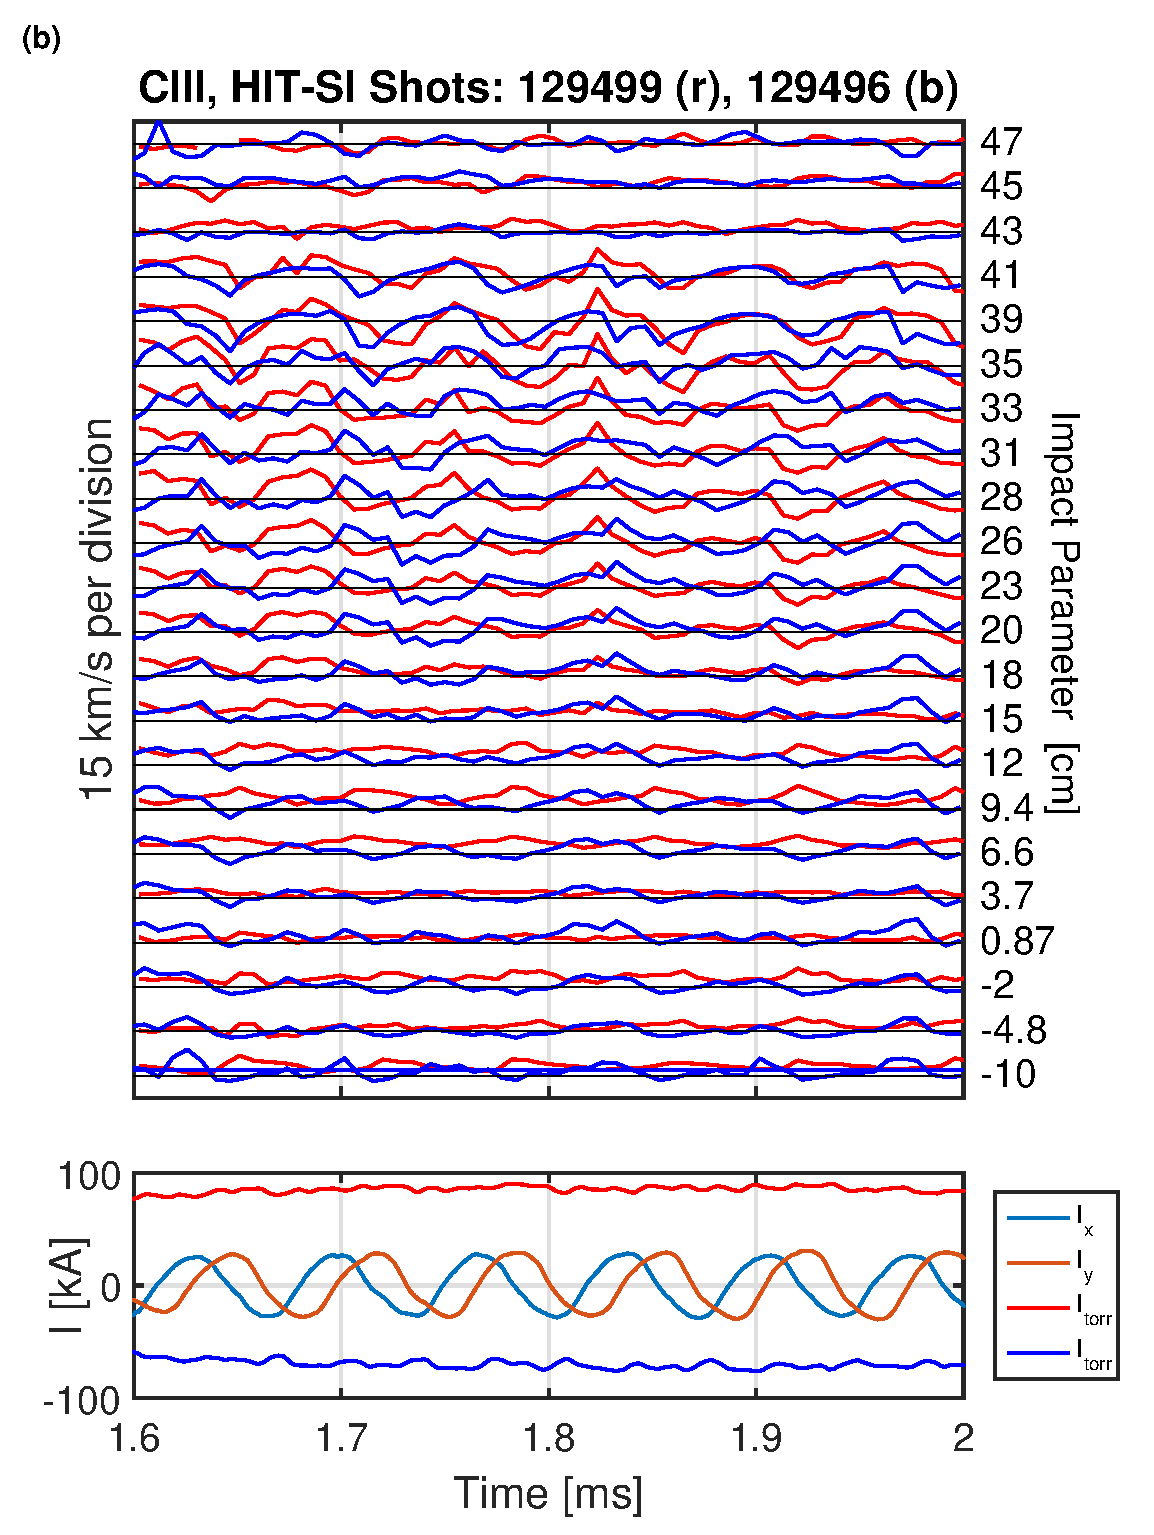
\includegraphics[width=3in]{129499_Lines_5}\caption{(a): Temperature from HIT-SI3 shot 160728013 C III line with injector and toroidal currents. (b): Velocity from HIT-SI shots 129499 (red) and 129496 (blue), C III line, with toroidal and injector currents. Black lines mark zero velocity for each chord. Data is missing where a gaussian could not be fit.}\label{Fig::Raw_VelTemp}
\end{figure*}
Most experiments cited previously, including HIT-SI \cite{Hossack_HitSi3}, have focused their analysis on the raw velocity and temperature data to extract flow and temperature profiles. This study improves upon this by isolating the component of the ion motion oscillating at the helicity injection frequency by fitting to a sinusoidal function. The initial parameter estimate is generated by a Fast Fourier Transform (FFT) of the data. Note that in contrast to BD, the dominant basis functions are expected to be periodic (if not sinusoidal), based on the periodic perturbation applied by the injectors. The data can be reconstructed, and additional information extracted, particularly the temporal phase. The functional form of the $i^{th}$ channel reconstructed velocity is:
\begin{equation}\label{Eqn::Fit_Fn}
v_i(t)=O_i+A_i\,\mathrm{\sin}(2{\pi}\:t\:f_{inj}+\phi_i)
\end{equation}
\begin{figure}
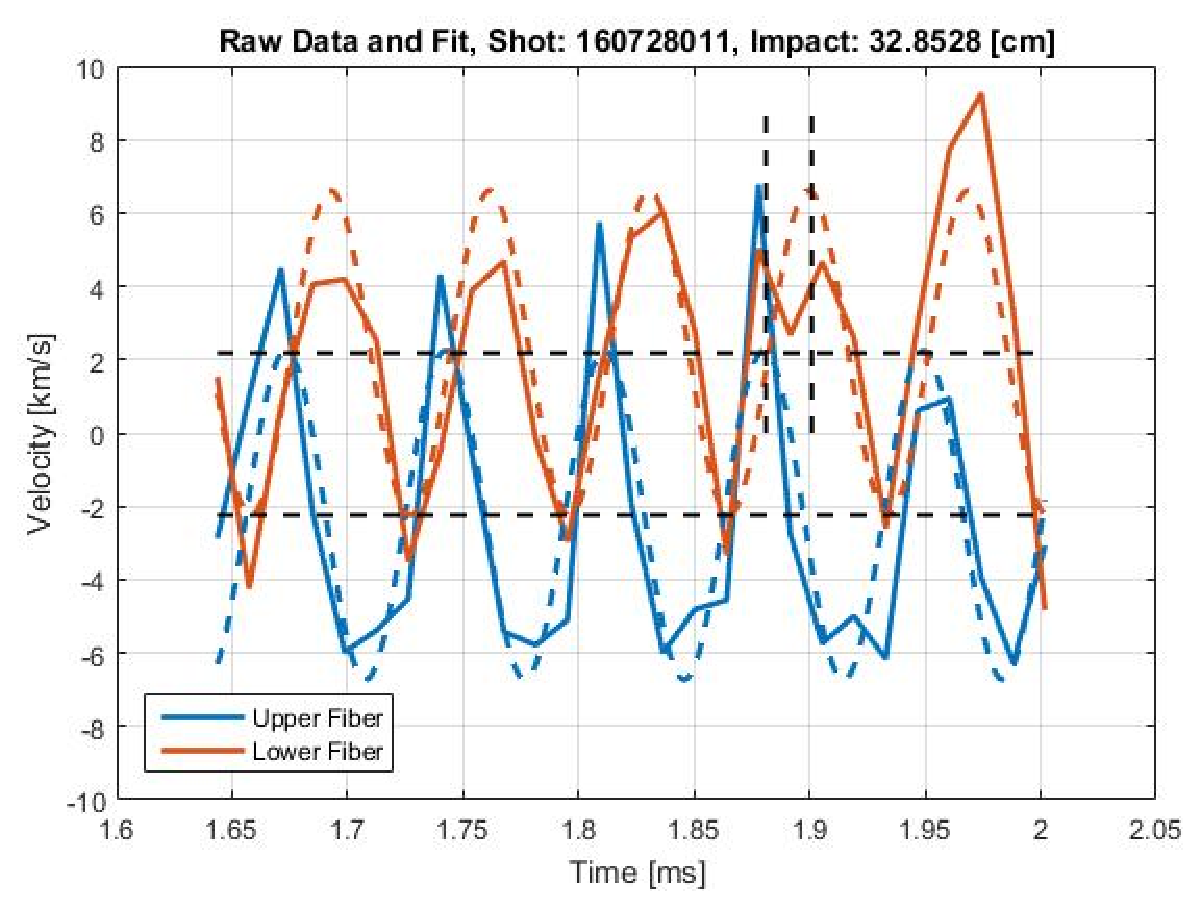
\includegraphics[width=3.5in]{ReconstExplain}\caption{Velocity reconstruction and visualization of analyzed quantities for HIT-SI3 shot 160728011, impact parameter $+$32.8 cm (blue) \& $-$32.8 cm (orange). Solid lines are raw data, dashed line is functional fit. Horizontal black line is sine fit offset, vertical black line is phase offset.}\label{Fig::Reconst Explain}
\end{figure}
Where $O_i$ is the offset velocity, $A_i$ is the amplitude, and $\phi_i$ is the temporal phase offset. These quantities are illustrated in figure \ref{Fig::Reconst Explain}, which shows the sine-fit of the velocity data for corresponding chords at impact parameter 32.8 cm for HIT-SI3 shot 160728011. The differences in velocity offset, temporal phase, and amplitude are visible. While the injector frequency-correlated component of the signal in both temperature and velocity is obvious in figure \ref{Fig::Raw_VelTemp}, the validity of a single frequency fit is determined from the Fourier power spectrum of this component and its higher harmonics relative to all others, as shown in Fig.\ref{Fig::FFT Spect}.
\begin{center}
\begin{figure*}
%\includegraphics[width=6in]{160728011L2L1VelSpect}
\hspace*{-10ex}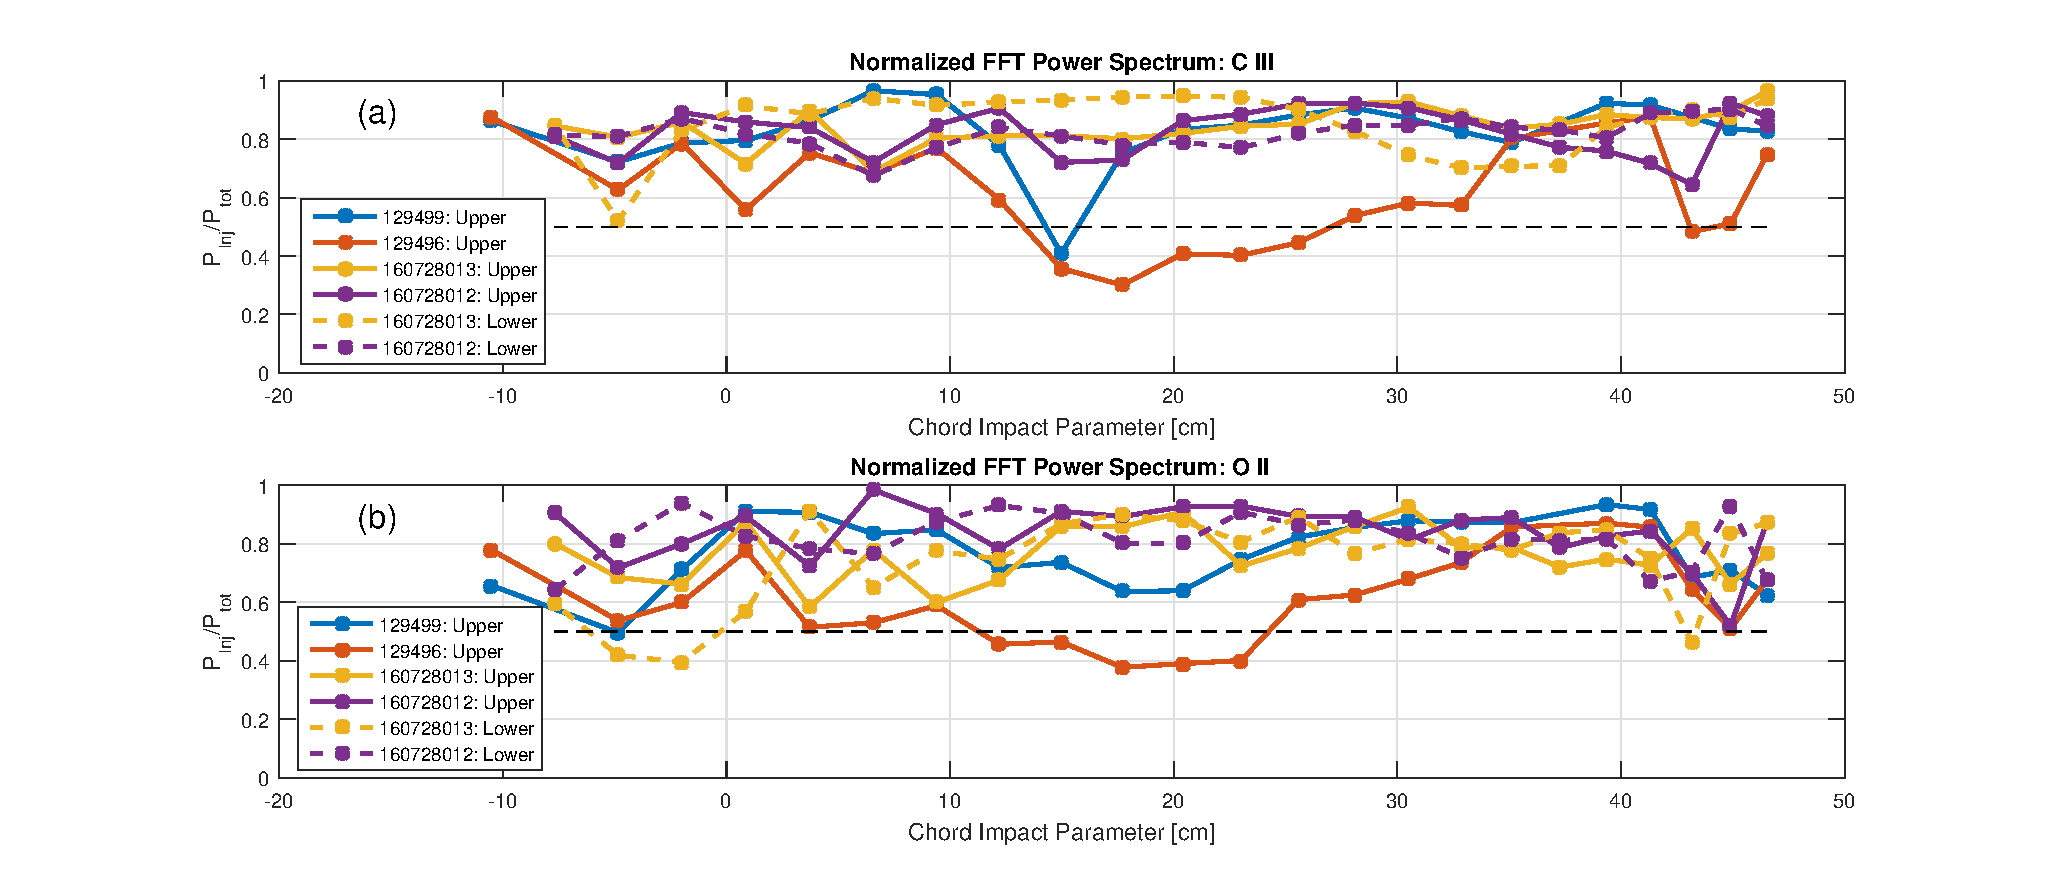
\includegraphics[width=8in]{FFT_3}\caption{Mode reconstruction: percentage of total FFT power spectrum contained at the injector frequency and up to three higher harmonics. All shots reported in Fig \ref{Fig::PosNeg_HIT-SI3} and \ref{Fig::PosNeg_HIT_SI} shown, C III in (a), O II in (b) for HIT-SI upper array and both HIT-SI3 arrays}\label{Fig::FFT Spect}
\end{figure*}
\end{center}



\subsection{Cycle-Averaged Calculated Quantities}\label{sec::CalcQuant}
From reconstructed data, the magnitude of the plasma displacement can be calculated from the magnitude of the velocity oscillation by analytic integration:
\begin{equation}
D_i=\frac{A_i}{{2\pi}\,f_{inj}}.
\end{equation}
Offset velocity $O_i$ is related to the toroidal flow, but can also be affected by calibration errors in $y_0$ from Eqn.\ref{Eqn::Gaussian}. On HIT-SI3, the dual-fiber views (Fig.\ref{Fibers Midplane}) allow the axisymmetric flow to be calculated as half the difference between velocity offsets of corresponding impact parameter above and below the geometric axis. HIT-SI did not have the lower viewport installed and so the velocity after injector shutoff was used to define ``zero velocity''.\\
\hspace*{4ex}The temporal phase $\phi$ describes temporal relationship between ion motion and injector current. On HIT-SI, phase is referenced from the zero crossing of the ``X'' injector (Fig \ref{Fig::V-Tank}b). On HIT-SI3, it is referenced from that of the ``A'' injector (Fig \ref{Fig::V-Tank}a). Phase correlations between channels suggest the extent of coherent structures in the plasma. In other words, regions of constant phase indicate that the plasma responds to the perturbation simultaneously.  In this analysis, two manipulations of the temporal displacement phase are performed. First, the phase of the upper fiber (the only array on HIT-SI) is decreased by $\pi$, so that the phase is now describing displacement in the positive toroidal direction rather than with respect to the detector. Second, the phase for negative current shots is decreased by $\pi$ for all channels, so that the phase is now describing plasma displacement in the toroidal current direction.   \\
\hspace*{4ex}The cycle-averaged temperature is given simply as the mean temperature as output by the Levenberg-Marquardt fitting to the raw data. The temperature also evolves in a semi-periodic fashion but no analysis of this oscillation has yet been attempted.

\subsection{Error Analysis}\label{sec:ErrorAnal}
\hspace*{4ex}The errors associated with the temperature, flow, and displacement profiles are calculated directly (Eqn. \ref{Eqn::ErrCal}) from the parameter error output by the Levenberg-Marquardt algorithm (sec \ref{sec::LM}), and the RMS error associated with the sine-fit (Eqn. \ref{Eqn::Fit_Fn}):
\begin{equation}\label{Eqn::ErrCal}
\begin{split}
\sigma_{T_j} = \sqrt{\frac{1}{T}\left(\frac{\sum_i^T\sigma_{T_{i,j}}^2}{T^2} + \mathrm{std(T(t))^2}\right)}\\
\sigma_{F_j}=\sqrt{\frac{1}{K\times{T}}\left(\sum_k^K\frac{\sum_i^T\sigma_{v,i,j,k}^2 }{T^2}+\sigma_{RMS,j,k}^2\right)}\\
\sigma_{D_{j,k}}=\sqrt{\frac{1}{T{\left(2\pi\times14500\right)^2}}\left(\frac{\sum_i^T\sigma_{v,i,j,k}^2}{T^2}+\sigma_{RMS,j}^2\right)}\\
\end{split}
\end{equation}
Where T is the number of time points which the fit is performed over, $\sigma_{v,i,j,k}$ is the LM calculated error associated with velocity for corresponding impacts $j$ from fiber array $k$ of $K$ ($K=1$ for HIT-SI) at timepoint $i$, $\sigma_{T_{i,j}}$ is the LM calculated error associated with temperature for chord $j$ and timepoint $i$, and $\sigma_{RMS}$ is the RMS error associated with the sine function fit.\\
\hspace*{4ex}We include the standard deviation of the temperature as an uncertainty to show the oscillation on top of the time-averaged profile. The addition of the sine fit RMS error extends the error bars in Fig \ref{Fig::PosNeg_HIT-SI3} and \ref{Fig::PosNeg_HIT_SI} slightly beyond the raw data error from Sec \ref{sec::LM}. This is done to show the temporal persistence of the profiles and fit. The $1/\sqrt{T}$ (where T is 59 for the HIT-SI shots and 46 for the HIT-SI3 shots analyzed here) term damps the errors and is primarily responsible for the error bars in Fig \ref{Fig::PosNeg_HIT-SI3} and \ref{Fig::PosNeg_HIT_SI} appearing small. The data in Fig \ref{Fig::PosNeg_HIT-SI3} (though not Fig \ref{Fig::PosNeg_HIT_SI}) has been previously published in\cite{Hossack_HitSi3}, however the error analysis techniques employed here are improved.  \\
\hspace*{4ex}The error associated with the temporal phase requires a different calculation: RMS error is assumed to be locally gaussian in the phase-parameter space, and the width of this gaussian is proportional to the associated error. Specifically, we perturb the phase of the fit $\pm\pi$, and compare the width of the resulting curve of RMS error to the curve produced by the same operation applied to the model being fit to itself. %Graphically, this is shown in Fig.\ref{Fig::Phase Error}. Note that the assumption of local gaussian error is clearly imperfect in the ideal error case.
%\begin{figure}
%\includegraphics[width=3in]{PhaseFitError}\caption{Calculation of Error Associated with Temporal Phase: Real and Ideal error describes changes in RMS error associated with perturbing Eqn \ref{Eqn::Fit_Fn} fit to the data and itself, respectively. Gaussian functions are fit to these curves.}\label{Fig::Phase Error}
%\end{figure}

%%%%%%%%%%%%%%%%%%%%%%%%%%%%%%%%%%%%%

\section{Results}
\hspace{4ex}The results of these operations are plotted to compare ion species (Fig.\ref{Fig::PosNeg_HIT-SI3} for C III,  Fig \ref{Fig::PosNeg_HIT_SI} for O II) and toroidal current direction (shots 129499 and 160726013 are positive, 129496 and 160728012 are negative) for both experiments. Other diagnostic traces for these shots are given in Fig \ref{Fig::Jscope}. The C III and O II lines listed on the plots are the 464.7 and 464.9 nm lines shown in Fig. \ref{HITSI_CCD}. The O II line is weaker, resulting in noisier data. Ion toroidal displacement phase, flow velocity, maximum displacement, and temperature profile are calculated as in Sec. \ref{sec::CalcQuant}, with error calculated as in Sec. \ref{sec:ErrorAnal}. The HIT-SI3 lower fiber array (Fig \ref{Fibers Midplane}) is plotted with dashed lines. The temporal phases of the injectors are given alongside the phase of the displacement.\\
\hspace*{4ex}The peaked temperature profile in C III varying between 10 and 40 eV  is observed for both experiments. Furthermore, in HIT-SI3, the overlap of the upper and lower fiber arrays indicates an axisymmetric mean temperature profile, roughly 8 eV hotter in positive toroidal current shots than negative shots of similar current magnitude. The shape of the O II temperature profile cannot be determined above error for HIT-SI or HIT-SI3, but is lower than C III for both.\\
\hspace*{4ex}The HIT-SI velocity profile cannot be determined for C III or O II due to high relative error. For HIT-SI3, however, we find a small but statistically significant axisymmetric flow of $\approx3$ km/s in negative current shots vs. $\approx1$ km/s for  positive current shots.\\
\hspace*{4ex}In HIT-SI, a relatively flat displacement phase region ($\Delta\phi\leq30^\circ$) is observed for positive current and both ion species, between $20\lesssim{R}\lesssim40$ cm. On HIT-SI3, a similar ``flat'' region is observed in the lower array (dashed lines), but not as much in the upper array. The inboard phase transition is not nearly as pronounced as in HIT-SI, and only appears in the upper array. On the outboard side, the two arrays show ion displacement locked to an injector (Fig. \ref{Fibers Midplane}).

\begin{figure*}
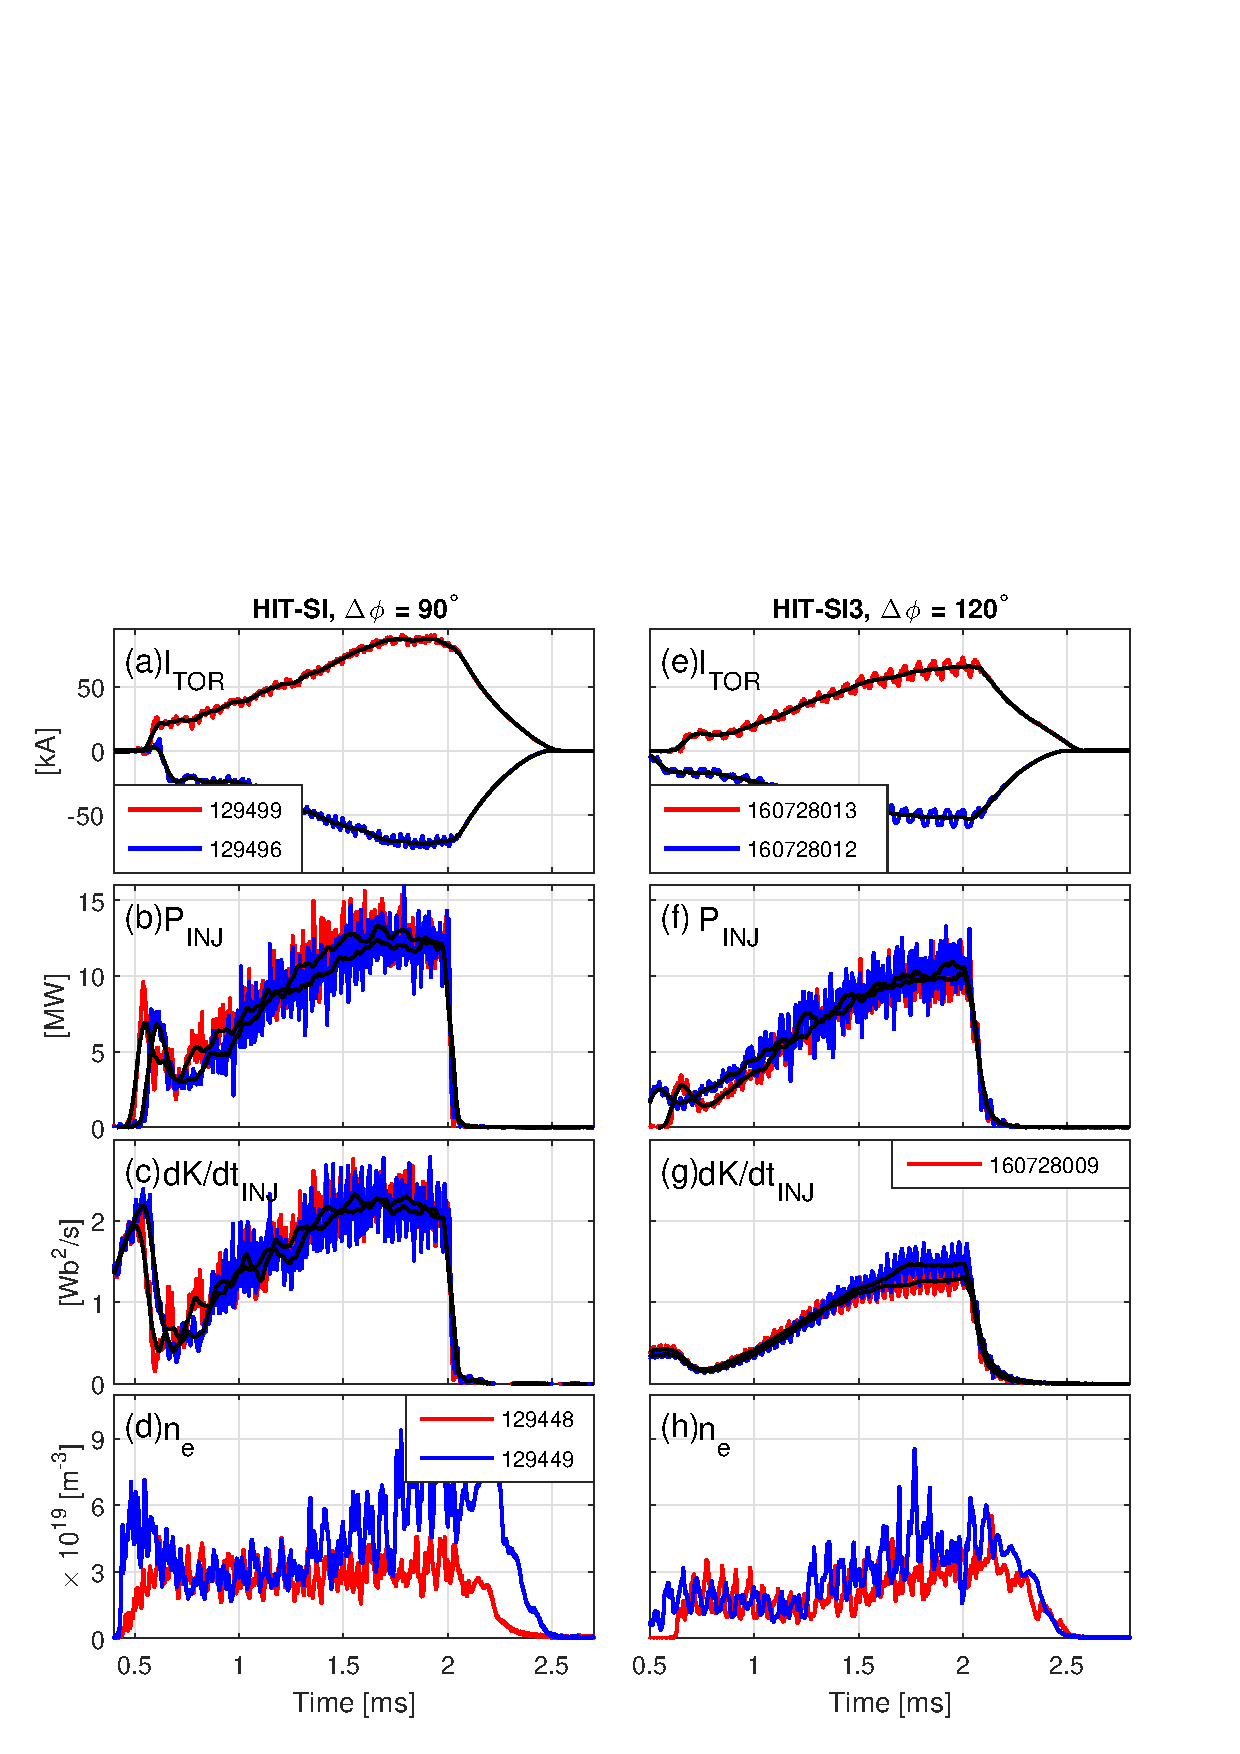
\includegraphics[width=6in]{Jscope5.jpg}\caption{Parameters of shots shown in Fig \ref{Fig::PosNeg_HIT-SI3} and \ref{Fig::PosNeg_HIT_SI}. Toroidal current (a,e), injector power (b,f), helicity injection rate , and electron density given. Data from similar shots substituted where unavailable in original, with small timebase shifts for consistency. Black line represents signal smoothed at the injector frequency.}\label{Fig::Jscope}
\end{figure*}

\begin{figure*}
%\includegraphics[width=3in]{160525017L1Compare_extendedRange}\nolinebreak
%\includegraphics[width=3in]{160525017L2Compare_extendedRange}
\hspace*{-10ex}\includegraphics[width=7in]{C_III_Compare_1}\caption{C III comparison of toroidal current direction. HIT-SI: a-d, HIT-SI3: e-h. Toroidal displacement phase, toroidal flow, maximum displacement, and temperature profile given. Lower fiber array plotted with dashed line, upper array with solid line. Phase of injectors given in plot.}\label{Fig::PosNeg_HIT-SI3}
\end{figure*}
\begin{figure*}
%\includegraphics[width=3in]{129499_OII_ComparisonError_DataSuppression_2}\nolinebreak
%\includegraphics[width=3in]{129499_CIII_ComparisonError_DataSuppression_2}
\hspace*{-10ex}\includegraphics[width=7in]{O_II_Compare_1}\caption{O II comparison of toroidal current direction. HIT-SI: a-d, HIT-SI3: e-h. Toroidal displacement phase, toroidal flow, maximum displacement, and temperature profile given. Lower fiber array plotted with dashed line, upper array with solid line. Phase of injectors given in plot.}\label{Fig::PosNeg_HIT_SI}
\end{figure*}


%%%%%%%%%%%%%%%%%%%%%%%%%%%%%%%%%%%%%%%%%%%%%%%%%%%%%%%%%%
\section{Discussion}
\hspace{4ex}The disparity in temperature between C III and O II on both experiments may indicate that the ion species density profile is not uniform, i.e.: O II may be relatively concentrated near the wall (due to its lower ionization energy) and C III may be concentrated near the core.  \\
\hspace*{4ex}A strong peak in the ion displacement of approximately 6 cm around impact parameter 40 cm is observed for C III and of approximately 4 cm for O II in both experiments. This is roughly consistent with the expected outboard separatrix location\cite{hossack2015study}. The decrease in displacement magnitude may be due to the decreased charge-to-mass ratio of O II vs C III. \\
\hspace*{4ex}The implications of the displacement phase are more complex. The ``flat'' phase region in HIT-SI (positive shot 129499) and the lower array in HIT-SI3 (both shots) implies that the spheromak is responding in a coherent manner to the applied perturbation. The almost $180^\circ$ phase transition between the inboard separatrix and the geometric axis on HIT-SI suggests that the spheromak is displacing the injector-linked plasma as it moves. These trends are not observed as clearly in O II due to noise. The phase behavior in HIT-SI appears to be flipped in the negative shot (129496). This implies that the opposite-current spheromak is responding in the opposite manner to injector flux which may be taking the same path. In HIT-SI3, the region of coherence is more pronounced in the upper fiber in the negative shot (160728012). The injector-locked motion between the geometric axis and the inner separatrix suggests that the observed displacement is either plasma being pulled around by the injector-linking plasma or is the injector plasma itself.\\
\hspace*{4ex}The temporal persistence of these profiles is indicated by relatively low RMS error in the sine fit and the FFT spectrum (Fig. \ref{Fig::FFT Spect}). Furthermore, the determination of chord and time-averaged mean ion temperature gradient (found on HIT-SI3 to be axisymmetric), the plasma displacement profile, and the temporal phase profile can be observed only due to the improved spatiotemporal resolution, and wide spatial extent. Prior IDS diagnostics could not fully resolve these profiles.

%\section{Sources of Error}
%\hspace*{4ex} %\textbf{EVERYTHING}
\section{Conclusions}
\hspace{4ex}An Ion Doppler Spectroscopy diagnostic system has been constructed which fulfills the requirements of sub-perturbation temporal resolution and high spatial resolution and extent on the HIT-SI and HIT-SI3 devices. Sub-injector timescale framerates (up to $10\times{14.5}$ kHz) on HIT-SI and full mid-plane viewing on HIT-SI3 with up to seventy-two spatial channels ($\leq2.8$ cm spatial resolution) have been produced for C III and O II impurities. Calibration, filtering, and fitting methods allow errors to be specified at $\lesssim1$ km/s and $\lesssim5$ eV, with an instrument temperature of 8-16 eV for C III. These improvements allow the determination of peaked, axisymmetric, chord-averaged temperature and displacement profiles on HIT-SI3, which agree with regions accessible to HIT-SI. Further, axisymmetric, current-dependent flow profiles have been found on HIT-SI3 of up to 3 km/s. Finally, coherent toroidal plasma displacement, locked to the applied perturbations, is seen in both experiments. Full midplane viewing, with high spatiotemporal resolution and parameter error analysis is not reported by other devices, making the accurate simultaneous observation of these profiles impossible. Future work includes moving the fiber arrays further out to the edge to better capture the edge-core transition. It is hoped that the advances in acquisition and analysis techniques presented here will prove beneficial to future researchers. 


\section{Acknowledgments}
The authors would like to acknowledge the assistance of the rest of the HIT-SI team: Kyle Morgan, Derek Sutherland, James Penna, Roy Taylor, Brian Nelson, John Rogers, and Jon Hayward. The authors would further like to acknowledge Professor Masayoshi Nagata of the University of Hyogo for the long term loan of the spectrometer.
\begin{comment}

Possible Topics for discussion:
\begin{enumerate}
\item Positive vs Negative current (Check)
\item Comparison of Temperature Evolution to Model
\item Velocity oscillations/Separatrix position calculation (kinda Check)
\item Comparison to Simulation (In forthcomming paper)
\item Different Frequency/Phasing (Incomparable? no HF HITSI3 data?)
\item OII vs CIII (we have the ability to do this)
\item Radial Shift Due to Flow
\item Beta

\item Analysis from the raw data (without FFT)
\item Analysis with FFT (contained in previous paper)
\end{enumerate}
\end{comment}


%%%%%%%%%%%%%%%%%%%%%%%%%%%%%%%%%%%%%%%%%%%%%%%%
%\newpage
\section{References}



%\bibliographystyle{unsrt}
\bibliography{Bibleography}
\begin{comment}
\begin{thebibliography}{}
% Fitting to Data References
\bibitem{1} \begin{verbatim}http://www.sciencedirect.com/science/article/pii/S0022407300001230}\end{verbatim}
\bibitem{2}\begin{verbatim}http://iopscience.iop.org/article/10.1088/0029-5515/22/6/009/meta\end{verbatim}
\bibitem{3}\begin{verbatim}http://iopscience.iop.org/article/10.1088/0029-5515/55/2/023009/meta\end{verbatim}
\bibitem{4}\begin{verbatim}http://iopscience.iop.org/article/10.1088/0741-3335/54/10/105022/meta\end{verbatim}
\bibitem{5}\begin{verbatim}http://www.euro-fusionscipub.org/wp-content/uploads/2014/11/EFDC020302.pdf\end{verbatim}
\bibitem{6}\begin{verbatim}http://aip.scitation.org/doi/full/10.1063/1.4891977\end{verbatim}
\bibitem{7}\begin{verbatim}http://aip.scitation.org/doi/10.1063/1.4758281\end{verbatim}
\bibitem{8}\begin{verbatim}http://iopscience.iop.org/article/10.1088/1742-6596/666/1/012002/pdf\end{verbatim}
\bibitem{9}\begin{verbatim}http://epubs.siam.org/doi/pdf/10.1137/0111030\end{verbatim}
\bibitem{10}\begin{verbatim}http://www.jstor.org/stable/43633451?seq=1#page_scan_tab_contents\end{verbatim}
\bibitem{11}\begin{verbatim}http://link.springer.com/article/10.1007/s00607-004-0083-1\end{verbatim}
\bibitem{12}Bamford, 1992
\bibitem{13}Hartog 1994
\bibitem{14}Rapisarda, 2007
\bibitem{15}\begin{verbatim}http://www.apmath.spbu.ru/cnsa/pdf/monograf/Numerical_Optimization2006.pdf\end{verbatim}
\bibitem{16}Numerical recipies in C
\bibitem{17}\begin{verbatim}http://onlinelibrary.wiley.com/doi/10.1002/9780470824566.app1/pdf\end{verbatim}

% Experimental Setup
\bibitem{18}AARONS THESIS

% BD filtering
\bibitem{19}\begin{verbatim}http://aip.scitation.org/doi/pdf/10.1063/1.1321739\end{verbatim}
\bibitem{20}\begin{verbatim}http://aip.scitation.org/doi/pdf/10.1063/1.870481\end{verbatim}
\bibitem{21}\begin{verbatim}http://aip.scitation.org/doi/pdf/10.1063/1.872796\end{verbatim}
\end{thebibliography}}

\end{comment}

\end{document}
